\chapter{Writing Cookbooks}

A cookbook is the fundamental unit of configuration and policy distribution. Each cookbook defines a scenario, such as everything needed to install and configure MySQL, and then it contains all of the components that are required to support that scenario.

As you read from previous chapter vendor cookbooks can help you to install and configure any possible software, but in most cases it is not enough. This is because you have your application, which need install, configure special cases only for this application. What is why you must to know how to write own Chef cookbooks.

Chef cookbooks is written on \href{https://www.ruby-lang.org}{Ruby} language. It is dynamic and open source programming language, which very well fit to use as \href{http://en.wikipedia.org/wiki/Domain-specific\_language}{DSL} for Chef recipes. Before you start reading this chapter, you should know Ruby at least basic stuff (Ruby types, loops, conditions, ERB, etc).

\section{Cookbook file organization}

For beginning we will generate cokbook by knife or berks. You can install both by bundler (we already did this in our kitchens). So, let's create <<my\_cool\_app>> cookbook:

\begin{lstlisting}[language=Bash,label=lst:cookbook-organization1]
$ cd site-cookbooks
$ knife cookbook create my_cool_app -o .
# or another way by berks
$ berks cookbook my_cool_app
\end{lstlisting}

After this you should see inside <<site-cookbooks>> new folder <<my\_cool\_app>>. This is our cookbook, which have such file structure inside:

\begin{lstlisting}[language=Bash,label=lst:cookbook-organization2]
$ ls -l my_cool_app
total 72
drwxr-xr-x  .
drwxr-xr-x  ..
drwxr-xr-x  .git
-rw-r--r--  .gitignore
-rw-r--r--  Berksfile
-rw-r--r--  Gemfile
-rw-r--r--@ LICENSE
-rw-r--r--  README.md
-rw-r--r--  Thorfile
-rw-r--r--  Vagrantfile
drwxr-xr-x  attributes
-rw-r--r--  chefignore
drwxr-xr-x  definitions
drwxr-xr-x  files
drwxr-xr-x  libraries
-rw-r--r--  metadata.rb
drwxr-xr-x  providers
drwxr-xr-x  recipes
drwxr-xr-x  resources
drwxr-xr-x  templates
\end{lstlisting}

Let's consider this structure:

\begin{itemize}
  \item \textbf{.git} - git repository skeleton (no need to do <<git init>>)
  \item \textbf{.gitignore} - specifies intentionally untracked files to ignore by Git
  \item \textbf{Berksfile} - file with cookbook dependencies for berkshelf (used for testing)
  \item \textbf{Gemfile} - file with gems for bundler (used for testing)
  \item \textbf{LICENSE} - file contain license information about cookbook
  \item \textbf{README.md} - file contains information about cookbook. <<.md>> mean \href{http://daringfireball.net/projects/markdown/syntax}{markdown} syntax
  \item \textbf{Thorfile} - file include tasks for thor gem (toolkit for building command-line interfaces, used for testing)
  \item \textbf{Vagrantfile} - file describe the type of machine required for a cookbook for vagrant
  \item \textbf{attributes} - this folder contain ruby files with default cookbook attributes, which you can redefine in environment, role or node attributes
  \item \textbf{chefignore} - specifies intentionally untracked files to ignore by Chef, Knife
  \item \textbf{definitions} - this folder contain ruby files which is used to declare resources so they can be added to the resource collection
  \item \textbf{files} - this folder contain files, which just need transfer to node (used by command <<cookbook\_file>>)
  \item \textbf{libraries} - this folder contain ruby files with Ruby code to be included in a cookbook, either as a way to extend the classes used by the chef-client or to implement a new class directly
  \item \textbf{metadata.rb} - a file, which contain all information (metadata) about the cookbook: name, dependencies, etc. (it is like gemset for ruby gems, package.json for npm, etc)
  \item \textbf{providers} - this folder contain providers for chef resources
  \item \textbf{recipes} - this folder contain recipes of this cookbook
  \item \textbf{resources} - this folder contain resources for chef (like build-in cron, deploy, etc)
  \item \textbf{templates} - this folder contain files written in a markup language that allows the contents of a file to be dynamically generated based on variables or complex logic. Used an Embedded Ruby (ERB) templates.
\end{itemize}

\section{Metadata}

Metadata is file, which contain all main information about cookbook. Let's consider our generated example:

\begin{lstlisting}[label=lst:cookbook-metadata1,title=my-server-cloud/site-cookbooks/my\_cool\_app/metadata.rb]
name             'my_cool_app'
maintainer       'YOUR_NAME'
maintainer_email 'YOUR_EMAIL'
license          'All rights reserved'
description      'Installs/Configures my_cool_app'
long_description IO.read(File.join(File.dirname(__FILE__), 'README.md'))
version          '0.1.0'
\end{lstlisting}

This file written on Ruby and can have such settings:

\begin{itemize}
  \item \textbf{name} - the name of the cookbook
  \item \textbf{maintainer} - the name of the person responsible for maintaining a cookbook, either an individual or an organization
  \item \textbf{maintainer\_email} - the email address for the person responsible for maintaining a cookbook. Only one email can be listed here
  \item \textbf{license} - the type of license under which a cookbook is distributed: <<Apache v2.0>>, <<GPL v2>>, <<GPL v3>>, <<MIT>>, or license <<Proprietary - All Rights Reserved>> (default)
  \item \textbf{description} - a short description of a cookbook and its functionality
  \item \textbf{long\_description} - a longer description that ideally contains full instructions on the proper use of a cookbook, including definitions, libraries, dependencies, and so on. In example the contents pulled from <<README.md>> file
  \item \textbf{version} - the current version of a cookbook. Version numbers always follow a simple three-number version sequence
  \item \textbf{attribute} - the list of attributes that are required to configure a cookbook
  \item \textbf{depends} - indicates that a cookbook has a dependency on another cookbook
  \item \textbf{recommends} - adds a dependency on another cookbook that is recommended, but not required
  \item \textbf{suggests} - adds a dependency on another cookbook that is suggested, but not required
  \item \textbf{conflicts} - indicates that a cookbook conflicts with another cookbook or cookbook version
  \item \textbf{grouping} - adds a title and description to a group of attributes within a namespace
  \item \textbf{provides} - adds a recipe, definition, or resource that is provided by this cookbook, should the auto-populated list be insufficient
  \item \textbf{recipe} - a description for a recipe, mostly for cosmetic value within the server user interface
  \item \textbf{replaces} - indicates that this cookbook should replace another (and can be used in-place of that cookbook)
  \item \textbf{supports} - indicates that a cookbook has a supported platform
\end{itemize}

For our cookbook we need little modify it:

\begin{lstlisting}[label=lst:cookbook-metadata2,title=my-server-cloud/site-cookbooks/my\_cool\_app/metadata.rb]
name             'my_cool_app'
maintainer       'Alexey Vasiliev'
maintainer_email 'leopard_ne@inbox.ru'
license          'MIT'
description      'Installs/Configures my_cool_app'
long_description IO.read(File.join(File.dirname(__FILE__), 'README.md'))
version          '0.1.0'
\end{lstlisting}

As of writing this cookbook, we will be adding information to this file on it.

\section{Resources and Providers}
\label{sec:cookbook-resources}

As you read from previous chapter, Chef inside have resources (in example we used \inline!package! resource). A resource defines the actions that can be taken, such as when a package should be installed, whether a service should be enabled or restarted, which groups, users, or groups of users should be created, where to put a collection of files, what the name of a new directory should be, and so on. During a chef-client run, each resource is identified and then associated with a provider. The provider then does the work to complete the action defined by the resource. Each resource is processed in the same order as they appear in a recipe. The chef-client ensures that the same actions are taken the same way everywhere and that actions produce the same result every time. A resource is implemented within a recipe using Ruby.

Let's look at the most necessary resources.

\subsection{Bash}

The bash resource is used to execute scripts using the Bash interpreter and includes all of the actions and attributes that are available to the execute resource. Example:

\begin{lstlisting}[label=lst:cookbook-resources-bash]
bash "install_something" do
  user "root"
  cwd "/tmp"
  code <<-EOH
  wget http://www.example.com/tarball.tar.gz
  tar -zxf tarball.tar.gz
  cd tarball
  ./configure
  make
  make install
  EOH
end
\end{lstlisting}

\subsection{Cron}

The cron resource is used to manage cron entries for time-based job scheduling. Attributes for a schedule will default to * if not provided. The cron resource requires access to a crontab program, typically cron. Example:

\begin{lstlisting}[label=lst:cookbook-resources-cron1]
cron "name_of_cron_entry" do
  hour "8"
  weekday "6"
  mailto "admin@opscode.com"
  action :create
end
\end{lstlisting}

\begin{lstlisting}[label=lst:cookbook-resources-cron2]
cron "noop" do
  hour "5"
  minute "0"
  command "/bin/true"
end
\end{lstlisting}

\subsection{Directory}

The directory resource is used to manage a directory, which is a hierarchy of folders that comprises all of the information stored on a computer. The root directory is the top-level, under which the rest of the directory is organized. The directory resource uses the name attribute to specify the path to a location in a directory. Typically, permission to access that location in the directory is required. Example:

\begin{lstlisting}[label=lst:cookbook-resources-directory1]
directory "/tmp/something" do
  owner "root"
  group "root"
  mode 00755
  action :create
end
\end{lstlisting}

\begin{lstlisting}[label=lst:cookbook-resources-directory2]
%w{dir1 dir2 dir3}.each do |dir|
  directory "/tmp/mydirs/#{dir}" do
    mode 00775
    owner "root"
    group "root"
    action :create
    recursive true
  end
end
\end{lstlisting}

\subsection{Git}

The git resource is used to manage source control resources that exist in a git repository. git version 1.6.5 (or higher) is required to use all of the functionality in the git resource. Example:

\begin{lstlisting}[label=lst:cookbook-resources-git1]
git "/opt/mysources/couch" do
  repository "git://git.apache.org/couchdb.git"
  reference "master"
  action :sync
end
\end{lstlisting}

\begin{lstlisting}[label=lst:cookbook-resources-git2]
git "#{Chef::Config[:file_cache_path]}/ruby-build" do
 repository "git://github.com/sstephenson/ruby-build.git"
 reference "master"
 action :sync
end

bash "install_ruby_build" do
 cwd "#{Chef::Config[:file_cache_path]}/ruby-build"
 user "rbenv"
 group "rbenv"
 code <<-EOH
   ./install.sh
   EOH
 environment 'PREFIX' => "/usr/local"
end
\end{lstlisting}

\subsection{Link}

The link resource is used to create symbolic or hard links. Example:

\begin{lstlisting}[label=lst:cookbook-resources-cookbook-link1]
link "/tmp/passwd" do
  to "/etc/passwd"
end
\end{lstlisting}

\begin{lstlisting}[label=lst:cookbook-resources-cookbook-link2]
link "/tmp/passwd" do
  to "/etc/passwd"
  link_type :hard
end
\end{lstlisting}

\subsection{Cookbook\_file}

The cookbook\_file resource is used to transfer files from a sub-directory of the files/ directory in a cookbook to a specified path that is located on the host running the chef-client or chef-solo. The file in a cookbook is selected according to file specificity, which allows different source files to be used based on the hostname, host platform (operating system, distro, or as appropriate), or platform version. Files that are located under COOKBOOK\_NAME/files/default can be used on any platform. Example:

\begin{lstlisting}[label=lst:cookbook-resources-cookbook-file1]
cookbook_file "/tmp/testfile" do
  source "testfile"
  mode 00644
end
\end{lstlisting}

\begin{lstlisting}[label=lst:cookbook-resources-cookbook-file2]
cookbook_file "/etc/yum.repos.d/custom.repo" do
  source "custom"
  mode 00644
  notifies :run, "execute[create-yum-cache]", :immediately
  notifies :create, "ruby_block[reload-internal-yum-cache]", :immediately
end
\end{lstlisting}

\subsection{Template}

The template resource is used to manage file contents with an embedded Ruby (erb) template. This resource includes actions and attributes from the file resource. Template files managed by the template resource follow the same file specificity rules as the remote\_file and file resources. Example:

\begin{lstlisting}[label=lst:cookbook-resources-cookbook-template1]
template "/tmp/config.conf" do
  source "config.conf.erb"
end
\end{lstlisting}

\begin{lstlisting}[label=lst:cookbook-resources-cookbook-template2]
template "/tmp/somefile" do
  mode 00644
  source "somefile.erb"
  not_if {File.exists?("/etc/passwd")}
end
\end{lstlisting}

\subsection{Script}

The script resource is used to execute scripts using the specified interpreter (Bash, Csh, Perl, Python, or Ruby) and includes all of the actions and attributes that are available to the execute resource. Example:

\begin{lstlisting}[label=lst:cookbook-resources-cookbook-script1]
script "install_something" do
  interpreter "bash"
  user "root"
  cwd "/tmp"
  code <<-EOH
  wget http://www.example.com/tarball.tar.gz
  tar -zxf tarball.tar.gz
  cd tarball
  ./configure
  make
  make install
  EOH
end
\end{lstlisting}

\subsection{User}

The user resource is used to add users, update existing users, remove users, and to lock/unlock user passwords. Example:

\begin{lstlisting}[label=lst:cookbook-resources-cookbook-user1]
user "random" do
  supports :manage_home => true
  comment "Random User"
  uid 1234
  gid "users"
  home "/home/random"
  shell "/bin/bash"
  password "$1$JJsvHslV$szsCjVEroftprNn4JHtDi."
end
\end{lstlisting}

There are a number of encryption options and tools that can be used to create a password shadow hash. In general, using a strong encryption method like SHA-512 and the passwd command in the OpenSSL toolkit is a good approach, however the encryption options and tools that are available may be different from one distribution to another. The following examples show how the command line can be used to create a password shadow hash. When using the \inline!passwd! command in the OpenSSL tool:

\begin{lstlisting}[language=Bash,label=lst:cookbook-resources-cookbook-user2]
$ openssl passwd -1 "theplaintextpassword"
\end{lstlisting}

Another example:

\begin{lstlisting}[label=lst:cookbook-resources-cookbook-user3]
user "systemguy" do
  comment "system guy"
  system true
  shell "/bin/false"
end
\end{lstlisting}

\subsection{Deploy}

The deploy resource is used to manage and control deployments. This is a popular resource, but is also complex, having the most attributes, multiple providers, the added complexity of callbacks, plus four attributes that support layout modifications from within a recipe.

The deploy resource is modeled after \href{http://capistranorb.com/}{Capistrano}, a utility and framework for executing commands in parallel on multiple remote machines via SSH. The deploy resource is designed to behave in a way that is similar to the \inline!deploy! and \inline!deploy:migration! tasks in Capistrano.
\section{Recipes}

Any cookbook contains recipes. The default recipe inside cookbook have name <<default>>. Let's add our default recipe, which will install \href{http://git-scm.com/}{git}:

\begin{lstlisting}[label=lst:cookbook-recipes1,title=my-server-cloud/site-cookbooks/my\_cool\_app/recipes/default.rb]
#
# Cookbook Name:: my_cool_app
# Recipe:: default
#
# Copyright (C) 2014 Alexey Vasiliev
#
# MIT
#

package 'git'
\end{lstlisting}

As you can see, at the beginning of recipe we have comments about this recipe. Next we add resource <<package>> with argument <<git>>. The <<package>> resource is used to manage packages on the system. For example, on Debian or Ubuntu resource <<package>> will use <<apt-get>> command to install git on system.

Now you should add <<my\_cool\_app>> into run-list to use this cookbook:

\begin{lstlisting}[label=lst:cookbook-recipes2,title=my-server-cloud/nodes/second.example.com.json]
{
  "name": "second.example.com",
  "json_class": "Chef::Node",
  "chef_type": "node",
  "chef_environment": "development",
  "normal": {
    "fqdn": "10.33.33.35"
  },
  "default": {},
  "override": {},
  "run_list": [
    "role[chef-client]",
    "role[nginx]",
    "recipe[my_cool_app]"
  ]
}
\end{lstlisting}

If you using Chef Server, don't forget upload this cookbook and update node on Chef Server by knife.

\begin{lstlisting}[language=Bash,label=lst:cookbook-recipes3]
$ knife cookbook upload my_cool_app
Uploading my_cool_app    [0.1.0]
Uploaded 1 cookbook.
$ knife node from file nodes/second.example.com.json
Updated Node second.example.com!
// on real environment you will execute "knife ssh 'name:second.example.com' 'sudo chef-client' -i ../keys/production.pem -x ubuntu"
$ vagrant provision chef_second_client
INFO: Chef Run complete in 26.935610739 seconds
INFO: Running report handler
\end{lstlisting}

Let's install also \href{http://en.wikipedia.org/wiki/Network\_Time\_Protocol}{ntp} package in the same recipe. Because we have in recipe Ruby syntax, we can little \href{http://ru.wikipedia.org/wiki/Dont\_repeat\_yourself}{DRY} our code:

\begin{lstlisting}[label=lst:cookbook-recipes4,title=my-server-cloud/site-cookbooks/my\_cool\_app/recipes/default.rb]
%w(git ntp).each do |pack|
  package pack
end
\end{lstlisting}

Again upload cookbook and run chef-client:

\begin{lstlisting}[language=Bash,label=lst:cookbook-recipes5]
$ knife cookbook upload my_cool_app
Uploading my_cool_app    [0.1.0]
Uploaded 1 cookbook.
// on real environment you will execute "knife ssh 'name:second.example.com' 'sudo chef-client' -i ../keys/production.pem -x ubuntu"
$ vagrant provision chef_second_client
INFO: Chef Run complete in 26.935610739 seconds
INFO: Running report handler
$ vagrant ssh chef_second_client
...
vagrant@precise64:~$ ps ax | grep ntp
 1115 ?        Ss     0:00 /usr/sbin/ntpd -p /var/run/ntpd.pid -g -u 103:108
13839 pts/2    S+     0:00 grep --color=auto ntp
vagrant@precise64:~$ git --version
git version 1.7.9.5
\end{lstlisting}

As you can see our simple cookbook is working.


\subsection{Assign Dependencies}

If a cookbook has a dependency on a recipe that is located in another cookbook, that dependency must be declared in the metadata.rb file for that cookbook using the depends keyword.

For example, if the following recipe is included in a cookbook named <<my\_app>>:

\begin{lstlisting}[language=Bash,label=lst:cookbook-recipes6]
include_recipe "apache2::mod_ssl"
\end{lstlisting}

Then the metadata.rb file for that cookbook would have:

\begin{lstlisting}[language=Bash,label=lst:cookbook-recipes7]
depends "apache2"
\end{lstlisting}

\subsection{Create Exceptions}

A recipe can write events to a log file and can cause exceptions using \inline{Chef::Log}. The levels include debug, info, warn, error, and fatal. For example, to just capture information:

\begin{lstlisting}[language=Bash,label=lst:cookbook-recipes7]
Chef::Log.info('some useful information')
\end{lstlisting}

Or to trigger a fatal exception:

\begin{lstlisting}[language=Bash,label=lst:cookbook-recipes8]
Chef::Log.fatal!('something bad')
\end{lstlisting}

\subsection{Include Recipes}

A recipe can include one (or more) recipes located in external cookbooks by using the \inline{include_recipe} method. When a recipe is included, the resources found in that recipe will be inserted (in the same exact order) at the point where the \inline{include_recipe} keyword is located. The syntax for including a recipe is like this:

\begin{lstlisting}[language=Bash,label=lst:cookbook-recipes9]
include_recipe "recipe"
\end{lstlisting}

For example:

\begin{lstlisting}[language=Bash,label=lst:cookbook-recipes10]
include_recipe "apache2::mod_ssl"
\end{lstlisting}

If the \inline{include_recipe} method is used more than once to include a recipe, only the first inclusion is processed and any subsequent inclusions are ignored.

\subsection{Reload Attributes}

Attributes sometimes depend on actions taken from within recipes, so it may be necessary to reload a given attribute from within a recipe. For example:

\begin{lstlisting}[language=Bash,label=lst:cookbook-recipes11]
ruby_block 'some_code' do
  block do
    node.from_file(run_context.resolve_attribute("COOKBOOK_NAME", "ATTR_FILE"))
  end
  action :nothing
end
\end{lstlisting}

\subsection{Accessor Methods}

Attribute accessor methods are automatically created and the method invocation can be used interchangeably with the keys. For example:

\begin{lstlisting}[language=Bash,label=lst:cookbook-recipes12]
default.apache.dir          = "/etc/apache2"
default.apache.listen_ports = [ "80","443" ]
ion :nothing
end
\end{lstlisting}

This is a matter of style and preference for how attributes are reloaded from recipes, and may be seen when retrieving the value of an attribute.
\section{Attributes}
\label{sec:cookbook-attributes}

An attribute can be defined in a cookbook (or a recipe) and then used to override the default settings on a node. When a cookbook is loaded during a chef-client run, these attributes are compared to the attributes that are already present on the node. When the cookbook attributes take precedence over the default attributes, the chef-client will apply those new settings and values during the chef-client run on the node.

An attribute file is located in the \inline{attributes/} sub-directory for a cookbook. When a cookbook is run against a node, the attributes contained in all attribute files are evaluated in the context of the node object. Node methods (when present) are used to set attribute values on a node. For example, the <<apache2>> cookbook contains an attribute file called \inline{default.rb}, which contains the following attributes:

\begin{lstlisting}[label=lst:cookbook-attributes1]
default["apache"]["dir"]          = "/etc/apache2"
default["apache"]["listen_ports"] = [ "80","443" ]
\end{lstlisting}

The use of the node object (node) is implicit in the previous example; the following example defines the node object itself as part of the attribute:

\begin{lstlisting}[label=lst:cookbook-attributes2]
node.default["apache"]["dir"]          = "/etc/apache2"
node.default["apache"]["listen_ports"] = [ "80","443" ]
\end{lstlisting}

In our cookbook <<my\_cool\_app>> we want create directory for web app, add to this directory html file, generate config for nginx and enable this configuration. Let's add all this by using Chef attributes and resources.

\begin{lstlisting}[label=lst:cookbook-attributes3,title=my-server-cloud/site-cookbooks/my\_cool\_app/attributes/default.rb]
default['my_cool_app']['web_dir']       = '/var/www/my_cool_app'
default['my_cool_app']['user']          = 'vagrant'
default['my_cool_app']['name']          = 'my_cool_app'
\end{lstlisting}

\begin{lstlisting}[label=lst:cookbook-attributes4,title=my-server-cloud/site-cookbooks/my\_cool\_app/recipes/default.rb]
# install needed package
%w(git ntp).each do |pack|
  package pack
end

# create directory for web app
directory node['my_cool_app']['web_dir'] do
  owner node['my_cool_app']['user']
  mode "0755"
  recursive true
end

# upload index.html file to web app directory as index.html
cookbook_file "#{node['my_cool_app']['web_dir']}/index.html" do
  owner node['my_cool_app']['user']
  source "index.html"
  mode 0755
end

# create nginx config from temlate nginx.conf.erb
nginx_config = "#{node['nginx']['dir']}" +
  "/sites-available/#{node['my_cool_app']['name']}.conf"
template nginx_config do
  source "nginx.conf.erb"
  mode "0644"
end

# activate nginx.conf in nginx
nginx_site "#{node['my_cool_app']['name']}.conf"
\end{lstlisting}

\begin{lstlisting}[language=HTML,label=lst:cookbook-attributes5,title=my-server-cloud/site-cookbooks/my\_cool\_app/templates/default/nginx.conf.erb]
server {
    listen 80 default;
    charset utf-8;
    root <%= node['my_cool_app']['web_dir'] %>;
}
\end{lstlisting}

\begin{lstlisting}[language=HTML,label=lst:cookbook-attributes6,title=my-server-cloud/site-cookbooks/my\_cool\_app/files/default/index.html]
<!DOCTYPE html>
<html lang="en">
<head>
  <meta charset="utf-8" />
  <meta http-equiv="X-UA-Compatible" content="IE=edge" />
  <title>My cool app</title>
  <meta name="viewport" content="width=device-width, initial-scale=1.0, user-scalable=0, maximum-scale=1.0" />
</head>
<body>
  <h1>This is my cool web app</h1>
</body>
</html>
\end{lstlisting}

\begin{lstlisting}[label=lst:cookbook-attributes7,title=my-server-cloud/site-cookbooks/my\_cool\_app/metadata.rb]
name             'my_cool_app'
maintainer       'Alexey Vasiliev'
maintainer_email 'leopard_ne@inbox.ru'
license          'MIT'
description      'Installs/Configures my_cool_app'
long_description IO.read(File.join(File.dirname(__FILE__), 'README.md'))
version          '0.1.0'

recipe 'my_cool_app',   'Configure my cool app'

depends 'nginx',           '~> 2.2.0'
\end{lstlisting}

As you can see, we add for default attributes for recipe. Better to use for cookbook attribute name as root for all attributes - in this case you will not have problem, if several cookbooks will use similar keys for settings. As you can see all attributes of this cookbook located inside <<my\_cool\_app>> attribute. In recipe we add needed commands to create and activate our index.html. Also we add to metadata information about recipe and dependence to nginx cookbook (because we used inside our recipe <<nginx\_site>> resource). After upload cookbook at Chef server and run chef-client at the second node, we can see results at \href{http://10.33.33.35}{http://10.33.33.35} (Pic~\ref{fig:my_cool_app_index}):

\begin{lstlisting}[language=Bash,label=lst:cookbook-attributes8]
$ knife cookbook upload my_cool_app
Uploading my_cool_app    [0.1.0]
Uploaded 1 cookbook.
// on real environment you will execute "knife ssh 'name:second.example.com' 'sudo chef-client' -i ../keys/production.pem -x ubuntu"
$ vagrant provision chef_second_client
...
INFO: directory[/var/www/my_cool_app] created directory /var/www/my_cool_app
INFO: directory[/var/www/my_cool_app] owner changed to 1000
INFO: directory[/var/www/my_cool_app] mode changed to 755
INFO: cookbook_file[/var/www/my_cool_app/index.html] created file /var/www/my_cool_app/index.html
INFO: cookbook_file[/var/www/my_cool_app/index.html] updated file contents /var/www/my_cool_app/index.html
INFO: cookbook_file[/var/www/my_cool_app/index.html] owner changed to 1000
INFO: cookbook_file[/var/www/my_cool_app/index.html] mode changed to 755
INFO: template[/etc/nginx/sites-available/my_cool_app.conf] created file /etc/nginx/sites-available/my_cool_app.conf
INFO: template[/etc/nginx/sites-available/my_cool_app.conf] updated file contents /etc/nginx/sites-available/my_cool_app.conf
INFO: template[/etc/nginx/sites-available/my_cool_app.conf] mode changed to 644
INFO: execute[nxensite my_cool_app.conf] ran successfully
INFO: execute[nxensite my_cool_app.conf] sending reload action to service[nginx] (delayed)
INFO: service[nginx] reloaded
...
\end{lstlisting}

\begin{figure}[ht!]
  \center{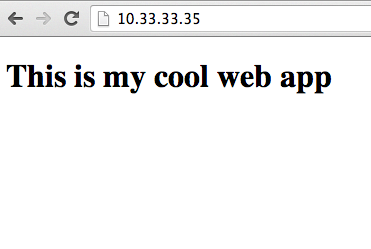
\includegraphics[width=0.6\textwidth]{my_cool_app_index}}
  \caption{Our cool app}
  \label{fig:my_cool_app_index}
\end{figure}
\section{Templates}

As you can see in previous chapter we used resource \inline{template} for generate nginx config in default recipe. A cookbook template is a file written in a markup language that allows the contents of a file to be dynamically generated based on variables or complex logic. Templates can contain Ruby expressions and statements. Templates are a great way to manage configuration files across an organization. A template requires a template resource being added to a recipe and then a corresponding Embedded Ruby (ERB) template being added to a cookbook.

To use a template, two things must happen:

\begin{itemize}
  \item A template resource must be added to a recipe
  \item An Embedded Ruby (ERB) template must be added to a cookbook
\end{itemize}

For example, the following template file and template resource settings can be used to manage a configuration file named \inline{/etc/sudoers}. Within a cookbook that uses sudo, the following resource could be added to \inline{recipes/default.rb}:

\begin{lstlisting}[label=lst:cookbook-templates1]
template "/etc/sudoers" do
  source "sudoers.erb"
  mode 0440
  owner "root"
  group "root"
  variables({
     :sudoers_groups => node[:authorization][:sudo][:groups],
     :sudoers_users => node[:authorization][:sudo][:users]
  })
end
\end{lstlisting}

And then create a template called \inline{sudoers.erb} and save it to \inline{templates/default/sudoers.erb}:

\begin{lstlisting}[label=lst:cookbook-templates2]
#
# /etc/sudoers
#
# Generated by Chef for <%= node[:fqdn] %>
#

Defaults        !lecture,tty_tickets,!fqdn

# User privilege specification
root          ALL=(ALL) ALL

<% @sudoers_users.each do |user| -%>
<%= user %>   ALL=(ALL) <%= "NOPASSWD:" if @passwordless %>ALL
<% end -%>

# Members of the sysadmin group may gain root privileges
%sysadmin     ALL=(ALL) <%= "NOPASSWD:" if @passwordless %>ALL

<% @sudoers_groups.each do |group| -%>
# Members of the group '<%= group %>' may gain root privileges
%<%= group %> ALL=(ALL) <%= "NOPASSWD:" if @passwordless %>ALL
<% end -%>
\end{lstlisting}

And then set the default attributes in \inline{attributes/default.rb}:

\begin{lstlisting}[label=lst:cookbook-templates3]
default["authorization"]["sudo"]["groups"] = [ "sysadmin","wheel","admin" ]
default["authorization"]["sudo"]["users"]  = [ "jerry","greg"]
\end{lstlisting}

When a template is rendered, Ruby expressions and statements are evaluated by the chef-client. The variables listed in the resource’s variables parameter and the node object are evaluated. The chef-client then passes these variables to the template, where they will be accessible as instance variables within the template; the node object can be accessed just as if it were part of a recipe, using the same syntax.

For example, a simple template resource like this:

\begin{lstlisting}[label=lst:cookbook-templates4]
node[:fqdn] = "latte"
template "/tmp/foo" do
  source "foo.erb"
  variables({
    :x_men => "are keen"
  })
end
\end{lstlisting}

And a simple Embedded Ruby (ERB) template like this:

\begin{lstlisting}[label=lst:cookbook-templates5]
The node <%= node[:fqdn] %> thinks the x-men <%= @x_men %>
\end{lstlisting}

Would render something like:

\begin{lstlisting}[label=lst:cookbook-templates6]
The node latte thinks the x-men are keen
\end{lstlisting}

Even though this is a very simple example, the full capabilities of Ruby can be used to tackle even the most complex and demanding template requirements.

\subsection{File Specificity}

A cookbook will frequently be designed to work across many platforms and will often be required to distribute a specific file to a specific platform. A cookbook can be designed to support distributing files across platforms, but ensuring that the right file ends up on each system.

The pattern for file specificity is as follows:

\begin{enumerate}
  \item \inline{host-node[:fqdn]}
  \item \inline{node[:platform]-node[:platform_version]}
  \item \inline{node[:platform]-version_components}: The version string is split on decimals and searched from greatest specificity to least; for example, if the location from the last rule was centos-5.7.1, then centos-5.7 and centos-5 would also be searched.
  \item \inline{node[:platform]}
  \item \inline{default}
\end{enumerate}

The naming of folders within cookbook directories must literally match the host notation used for template specificity matching. For example, if a host is named <<foo.example.com>>, then the folder must be named <<host-foo.example.com>>.

A cookbook may have a \inline{/templates} directory structure like this:

\begin{lstlisting}[language=Bash,label=lst:cookbook-templates7]
templates/
  windows-6.2
  windows-6.1
  windows-6.0
  windows
  default
\end{lstlisting}

and a resource that looks something like the following:

\begin{lstlisting}[label=lst:cookbook-templates8]
template "C:\path\to\file\text_file.txt" do
  source "text_file.txt"
  mode 0755
  owner "root"
  group "root"
end
\end{lstlisting}

This resource would be matched in the same order as the /templates directory structure. For a node named <<host-node-desktop>> that is running Windows 7, the second item would be the matching item and the location:

\begin{lstlisting}[language=Bash,label=lst:cookbook-templates8]
/templates
  windows-6.2/text_file.txt
  windows-6.1/text_file.txt
  windows-6.0/text_file.txt
  windows/text_file.txt
  default/text_file.txt
\end{lstlisting}

\subsection{Partial Templates}

A template can be built in a way that allows it to contain references to one (or more) smaller template files. (These smaller template files are also referred to as partials.) A partial can be referenced from a template file in one of the following ways:

\begin{itemize}
  \item By using the Ruby render method in the template file
  \item By using the template resource and the variables parameter
\end{itemize}

Use the render method in a template to reference a partial template file with the following syntax:

\begin{lstlisting}[language=Bash,label=lst:cookbook-templates9]
<%= render "partial_name.txt.erb", :option => {} %>
\end{lstlisting}

where \inline{partial_name.txt.erb} is the name of the partial template file and \inline{:option} is one (or more) of the following options:

\begin{itemize}
  \item \inline{:cookbook} - by default, a partial template file is assumed to be located in the cookbook that contains the top-level template. Use this option to specify the path to a different cookbook
  \item \inline{:local} - indicates that the name of the partial template file should be interpreted as a path to a file in the local file system or looked up in a cookbook using the normal rules for template files. Set to true to interpret as a path to a file in the local file system and to false to use the normal rules for template files
  \item \inline{:source} - by default, a partial template file is identified by its file name. Use this option to specify a different name or a local path to use (instead of the name of the partial template file)
  \item \inline{:variables} - a hash of \inline{variable_name => value} that will be made available to the partial template file. When this option is used, any variables that are defined in the top-level template that are required by the partial template file must have them defined explicitly using this option
\end{itemize}

For example:

\begin{lstlisting}[language=Bash,label=lst:cookbook-templates10]
<%= render "simple.txt.erb", :variables => {:user => @user }, :local => true %>
\end{lstlisting}


\section{LWRPs}
\label{sec:cookbook-lwrp}

A LWRP is a part of a cookbook that is used to extend the chef-client in a way that allows custom actions to be defined, and then used in recipes in much the same way as any platform resource. A LWRP has two principal components:

\begin{itemize}
  \item A lightweight resource that defines a set of actions and attributes
  \item A lightweight provider that tells the chef-client how to handle each action, what to do if certain conditions are met, and so on
\end{itemize}

In addition, most lightweight providers are built using platform resources and some lightweight providers are built using custom Ruby code.

Once created, a LWRP becomes a Ruby class within the organization. During each chef-client run, the chef-client will read the lightweight resources from recipes and process them alongside all of the other resources. When it is time to configure the node, the chef-client will use the corresponding lightweight provider to determine the steps required to bring the system into the desired state.

Where the lightweight resource represents a piece of the system, its current state, and the action that is needed to move it to the desired state, a lightweight provider defines the steps that are required to bring that piece of the system from its current state to the desired state. A LWRP behaves similar to platform resources and providers:

\begin{itemize}
  \item A lightweight resource is a key part of a recipe
  \item A lightweight resource defines the actions that can be taken
  \item During a chef-client run, each lightweight resource is identified, and then associated with a lightweight provider
  \item A lightweight provider does the work to complete the action requested by the lightweight resource
\end{itemize}

Lightweight resources and providers are loaded from files that are saved in the following cookbook sub-directories:

\begin{tabular}{ | l | l | }
  \hline
  Directory	& Description \\
  \hline
  providers/ & The sub-directory in which lightweight providers are located. \\
  resources/ & The sub-directory in which lightweight resources are located. \\
  \hline
\end{tabular}

The naming patterns of lightweight resources and providers are determined by the name of the cookbook and by the name of the files in the <<resources/>> and <<providers/>> sub-directories. For example, if a cookbook named <<example>> was downloaded to the chef-repo, it would be located at <</cookbooks/example/>>. If that cookbook contained two resources and two providers, the following files would be part of the <<resources/>> directory:

\begin{tabular}{ | l | l | l | }
  \hline
  Files	& Resource Name	& Generated Class \\
  \hline
  default.rb & example & Chef::Resource::Example \\
  custom.rb	& example\_custom & Chef::Resource::ExampleCustom \\
  \hline
\end{tabular}

And the following files would be part of the <<providers/>> directory:

\begin{tabular}{ | l | l | l | }
  \hline
  Files	& Provider Name	& Generated Class \\
  \hline
  default.rb & example & Chef::Provider::Example \\
  custom.rb	& custom & Chef::Provider::ExampleCustom \\
  \hline
\end{tabular}

Let's add in our <<my\_cool\_app>> LWRP, which will add in \inline{/etc/ssh/ssh_known_hosts} host.

\subsection{Resources}

First of all we should create direcotry <<resources>> and add to it \inline{know_host.rb} file with content:

\begin{lstlisting}[label=lst:cookbook-lwrp1,title=my-server-cloud/site-cookbooks/my\_cool\_app/resources/know\_host.rb]
actions :create, :delete
default_action :create

attribute :host, :kind_of => String, :name_attribute => true, :required => true
attribute :key, :kind_of => String
attribute :port, :kind_of => Fixnum, :default => 22
attribute :known_hosts_file, :kind_of => String, :default => '/etc/ssh/ssh_known_hosts'

# Needed for Chef versions < 0.10.10
def initialize(*args)
  super
  @action = :create
end
\end{lstlisting}

Let's take it line by line. The first line specifies the allowed actions. Actions are what your resource can do, e.g. start, stop, create, delete, etc. In this case, you can \inline{:create} or \inline{:delete} known host. The next line defines the \inline{default_action} for our resource, in this case \inline{:create}. If you don't specify an action when you use the resource in a recipe, it will default to creating a known host, which is what you probably want. A general philosophy of Chef is to define intelligent or <<sane>> defaults.

Lines 4-7 define attributes, or properties of the known host resource we are creating. Line 4 defines an \inline{:host} attribute. Its \inline{:name_attribute} is true, which means that this attribute will be set to the string between \inline{my_cool_app_know_host} and \inline{do}. Example:

\begin{lstlisting}[label=lst:cookbook-lwrp2]
my_cool_app_know_host "Add github host" do
  host 'github.com'
end

my_cool_app_know_host 'github.com' do
  # The :host attribute will be set to 'github.com'
end
\end{lstlisting}

In the second example above, the \inline{:host} attribute wll be set to <<github.com>>.

Also, on line 4, we are definining the \inline{kind_of} validation parameter to tell the resource which kind of data we should expect (in this case, a string), whether this attribute is required (yes). Line 5 defines a \inline{:key} attribute, which is an optional string with no default. Line 6 defines a \inline{:port} attribute, a Ruby Fixnum (i.e. an integer) with a default of 22, which is the default when you create a known host. Line 7 defines a \inline{:known_hosts_file} attribute, a string with a default of \inline{/etc/ssh/ssh_known_hosts}, which is the default file with known hosts for ssh client.

For example, the \inline{cron_d} lightweight resource (found in the cron cookbook) can be used to manage files located in \inline{/etc/cron.d}:

\begin{lstlisting}[label=lst:cookbook-lwrp3]
actions :create, :delete
default_action :create

attribute :name, :kind_of => String, :name_attribute => true
attribute :cookbook, :kind_of => String, :default => "cron"
attribute :minute, :kind_of => [Integer, String], :default => "*"
attribute :hour, :kind_of => [Integer, String], :default => "*"
attribute :day, :kind_of => [Integer, String], :default => "*"
attribute :month, :kind_of => [Integer, String], :default => "*"
attribute :weekday, :kind_of => [Integer, String], :default => "*"
attribute :command, :kind_of => String, :required => true
attribute :user, :kind_of => String, :default => "root"
attribute :mailto, :kind_of => [String, NilClass]
attribute :path, :kind_of => [String, NilClass]
attribute :home, :kind_of => [String, NilClass]
attribute :shell, :kind_of => [String, NilClass]
\end{lstlisting}

where

\begin{itemize}
  \item the \inline{actions} allow a recipe to manage entries in a crontab file (create entry, delete entry)
  \item \inline{:create} is the default action
  \item \inline{:minute}, \inline{:hour}, \inline{:day}, \inline{:month}, and \inline{:weekday} are the collection of attributes used to schedule a cron job, assigned a default value of <<*>>
  \item \inline{:command} is the command that will be run (and also required)
  \item \inline{:user} is the user by which the command is run
  \item \inline{:mailto}, \inline{:path}, \inline{:home}, and \inline{:shell} are optional environment variables that do not have default value, which each being defined as an array that supports the String and NilClass Ruby classes
\end{itemize}

\subsection{Providers}

Now we need to create file \inline{know_host.rb} in <<providers>> directory:

\begin{lstlisting}[label=lst:cookbook-lwrp3,title=my-server-cloud/site-cookbooks/my\_cool\_app/providers/know\_host.rb]
# Support whyrun
def whyrun_supported?
  true
end

action :create do
  key, comment = insure_for_file(new_resource)
  # Use a Ruby block to edit the file
  ruby_block "add #{new_resource.host} to #{new_resource.known_hosts_file}" do
    block do
      file = ::Chef::Util::FileEdit.new(new_resource.known_hosts_file)
      file.insert_line_if_no_match(/#{Regexp.escape(comment)}|#{Regexp.escape(key)}/, key)
      file.write_file
    end
  end
  new_resource.updated_by_last_action(true)
end

action :delete do
  key, comment = insure_for_file(new_resource)
  # Use a Ruby block to edit the file
  ruby_block "del #{new_resource.host} from #{new_resource.known_hosts_file}" do
    block do
      file = ::Chef::Util::FileEdit.new(new_resource.known_hosts_file)
      file.search_file_delete_line(/#{Regexp.escape(comment)}|#{Regexp.escape(key)}/)
      file.write_file
    end
  end
  new_resource.updated_by_last_action(true)
end

def insure_for_file(new_resource)
  key = (new_resource.key || `ssh-keyscan -H -p #{new_resource.port} #{new_resource.host} 2>&1`)
  comment = key.split("\n").first || ""

  Chef::Application.fatal! "Could not resolve #{new_resource.host}" if key =~ /getaddrinfo/

  # Ensure that the file exists and has minimal content (required by Chef::Util::FileEdit)
  file new_resource.known_hosts_file do
    action        :create
    backup        false
    content       '# This file must contain at least one line. This is that line.'
    only_if do
      !::File.exists?(new_resource.known_hosts_file) || ::File.new(new_resource.known_hosts_file).readlines.length == 0
    end
  end
  [key, comment]
end
\end{lstlisting}

\subsection{DSL Methods}

\subsubsection{action}

The action method is used to define the steps that will be taken for each of the possible actions defined by the lightweight resource. Each action must be defined in separate action blocks within the same file. The syntax for the action method is as follows:

\begin{lstlisting}[label=lst:cookbook-lwrp-dsl-action]
action :action_name do
  if @current_resource.exists
    Chef::Log.info "#{ @new_resource } already exists - nothing to do."
  else
    resource "resource_name" do
      Chef::Log.info "#{ @new_resource } created."
    end
  end
  new_resource.updated_by_last_action(true)
end
\end{lstlisting}

where:

\begin{itemize}
  \item \inline{:action_name} corresponds to an action defined by a lightweight resource
  \item if \inline{@current_resource.exists} is a condition test that is using an instance variable to see if the object already exists on the node; this is an example of a test for idempotence
  \item If the object already exists, a \inline{@new_resource} already exists - nothing to do. log entry is created
  \item If the object does not already exists, the resource block is run. This block is a recipe that tells the chef-client what to do. A \inline{@new_resource} created. log entry is created
\end{itemize}

\subsubsection{current\_resource}

The \inline{current_resource} method is used to represent a resource as it exists on the node at the beginning of the chef-client run. In other words: what the resource is currently. The chef-client compares the resource as it exists on the node to the resource that is created during the chef-client run to determine what steps need to be taken to bring the resource into the desired state. This method is often used as an instance variable (\inline{@current_resource}).

For example:

\begin{lstlisting}[label=lst:cookbook-lwrp-dsl-current-resource]
action :add do
  unless @current_resource.exists
    cmd = "#{appcmd} add app /site.name:\"#{@new_resource.app_name}\""
    cmd << " /path:\"#{@new_resource.path}\""
    cmd << " /applicationPool:\"#{@new_resource.application_pool}\"" if @new_resource.application_pool
    cmd << " /physicalPath:\"#{@new_resource.physical_path}\"" if @new_resource.physical_path
    Chef::Log.debug(cmd)
    shell_out!(cmd)
    Chef::Log.info("App created")
  else
    Chef::Log.debug("#{@new_resource} app already exists - nothing to do")
  end
end
\end{lstlisting}

where the \inline{unless} conditional statement checks to make sure the resource doesn't already exist on a node, and then runs a series of commands when it doesn't. If the resource already exists, the log entry would be <<Foo app already exists - nothing to do.>>

\subsubsection{load\_current\_resource}

The \inline{load_current_resource} method is used to find a resource on a node based on a collection of attributes. These attributes are defined in a lightweight resource and are loaded by the chef-client when processing a recipe during a chef-client run. This method will ask the chef-client to look on the node to see if a resource exists with specific matching attributes.

For example:

\begin{lstlisting}[label=lst:cookbook-lwrp-dsl-load-current-resource]
def load_current_resource
  @current_resource = Chef::Resource::TransmissionTorrentFile.new(@new_resource.name)
  Chef::Log.debug("#{@new_resource} torrent hash = #{torrent_hash}")
  path = "foo:#{@new_resource.att1}@#{@new_resource.att2}:#{@new_resource.att3}/path"
  @transmission = Opscode::Transmission::Client.new(path)
  @torrent = nil
  begin
    @torrent = @transmission.get_torrent(torrent_hash)
    info = "Found existing #{@new_resource} in swarm "+
    "with name of '#{@torrent.name}' and status of '#{@torrent.status_message}'"
    Chef::Log.info(info)
    @current_resource.torrent(@new_resource.torrent)
  rescue
    Chef::Log.debug("Cannot find #{@new_resource} in the swarm")
  end
  @current_resource
end
\end{lstlisting}

In the previous example, if a resource exists with matching attributes, the chef-client does nothing and if a resource does not exist with matching attributes, the chef-client will enforce the state declared in \inline{new_resource}.

\subsubsection{new\_resource}

The \inline{new_resource} method is used to represent a resource as loaded by the chef-client during the chef-client run. In other words: what the resource should be. The chef-client compares the resource as it exists on the node to the resource that is created during the chef-client run to determine what steps need to be taken to bring the resource into the desired state.

For example:

\begin{lstlisting}[label=lst:cookbook-lwrp-dsl-new-resource]
action :delete do
  if exists?
    if ::File.writable?(new_resource.path)
      Chef::Log.info("Deleting #{new_resource} at #{new_resource.path}")
      ::File.delete(new_resource.path)
      new_resource.updated_by_last_action(true)
    else
      raise "Cannot delete #{new_resource} at #{new_resource.path}!"
    end
  end
end
\end{lstlisting}

where the chef-client checks to see if the file exists, then if the file is writable, and then attempts to delete the resource. \inline{path} is an attribute of the new resource that is defined by the lightweight resource.

\subsubsection{updated\_by\_last\_action}

The \inline{updated_by_last_action} method is used to notify a lightweight resource that a node was updated successfully. For example, the \inline{cron_d} lightweight resource in the cron cookbook:

\begin{lstlisting}[label=lst:cookbook-lwrp-dsl-updated]
action :create do
  t = template "/etc/cron.d/#{new_resource.name}" do
    cookbook new_resource.cookbook
    source "cron.d.erb"
    mode "0644"
    variables({
        :name => new_resource.name,
        :minute => new_resource.minute,
        :hour => new_resource.hour,
        :day => new_resource.day,
        :month => new_resource.month,
        :weekday => new_resource.weekday,
        :command => new_resource.command,
        :user => new_resource.user,
        :mailto => new_resource.mailto,
        :path => new_resource.path,
        :home => new_resource.home,
        :shell => new_resource.shell
      })
    action :create
  end
  new_resource.updated_by_last_action(t.updated_by_last_action?)
end
\end{lstlisting}

where \inline{t.updated_by_last_action?} uses a variable to check whether a new crontab entry was created.

\subsubsection{use\_inline\_resources}

A lightweight resource should be set to inline compile mode by adding the \inline{use_inline_resources} method at the top of the provider. This ensures that notifications work properly across the resource collection. The \inline{use_inline_resources} method was added to the chef-client starting in version 11.0 to address the behavior described below. The \inline{use_inline_resources} method should be considered a requirement for any lightweight resource authored against the 11.0+ versions of the chef-client. This behavior will become the default behavior in an upcoming version of the chef-client.

\subsubsection{whyrun\_supported?}

why-run mode is a way to see what the chef-client would have configured, had an actual chef-client run occurred. This approach is similar to the concept of <<no-operation>> (or <<no-op>>): decide what should be done, but then don't actually do anything until it's done right. This approach to configuration management can help identify where complexity exists in the system, where inter-dependencies may be located, and to verify that everything will be configured in the desired manner.

When why-run mode is enabled, a chef-client run will occur that does everything up to the point at which configuration would normally occur. This includes getting the configuration data, authenticating to the server, rebuilding the node object, expanding the run list, getting the necessary cookbook files, resetting node attributes, identifying the resources, and building the resource collection and does not include mapping each resource to a provider or configuring any part of the system.

When the chef-client is run in why-run mode, certain assumptions are made:

\begin{itemize}
  \item If the service resource cannot find the appropriate command to verify the status of a service, why-run mode will assume that the command would have been installed by a previous resource and that the service would not be running
  \item For \inline{not_if} and \inline{only_if} attribute, why-run mode will assume these are commands or blocks that are safe to run. These conditions are not designed to be used to change the state of the system, but rather to help facilitate idempotency for the resource itself. That said, it may be possible that these attributes are being used in a way that modifies the system state
  \item The closer the current state of the system is to the desired state, the more useful why-run mode will be. For example, if a full run-list is run against a fresh system, that run-list may not be completely correct on the first try, but also that run-list will produce more output than smaller run-list
\end{itemize}

The \inline{whyrun_supported?} method is used to set a lightweight provider to support why-run mode. The syntax for the \inline{whyrun_supported?} method is as follows:

\begin{lstlisting}[label=lst:cookbook-lwrp-why-run]
def whyrun_supported?
  true
end
\end{lstlisting}

where \inline{whyrun_supported?} is set to true for any lightweight provider that supports using why-run mode. When why-run mode is supported by the a lightweight provider, the \inline{converge_by} method is used to define the strings that are logged by the chef-client when it is run in why-run mode.

\subsubsection{Log entries and rescue}

Use the \inline{Chef::Log} class in a lightweight provider to define log entries that are created during a chef-client run. The syntax for a log message is as follows:

\begin{lstlisting}[label=lst:cookbook-lwrp-logs1]
Chef::Log.log_type("message")
\end{lstlisting}

where

\begin{itemize}
  \item \inline{log_type} can be .debug, .info, .warn, .error, or .fatal
  \item <<message>> is the message that is logged
\end{itemize}

For example, from the <<repository.rb>> provider in the yum cookbook:

\begin{lstlisting}[label=lst:cookbook-lwrp-logs2]
action :add do
  unless ::File.exists?("/etc/yum.repos.d/#{new_resource.repo_name}.repo")
    Chef::Log.info "Adding #{new_resource.repo_name} repository to /etc/yum.repos.d/#{new_resource.repo_name}.repo"
    repo_config
  end
end
\end{lstlisting}

where the \inline{Chef::Log} class appends .info as the log type. If the name of the repo was <<foo>>, then the log message would be <<Adding foo repository to /etc/yum.repos.d/foo.repo>>.

Another example shows two log entries, one that is triggered when a service is being restarted, and then another that is triggered after the service has been restarted:

\begin{lstlisting}[label=lst:cookbook-lwrp-logs3]
action :restart do
  if @current_resource.running
    Chef::Log.debug "Restarting #{new_resource.service_name}"
    shell_out!(restart_command)
    new_resource.updated_by_last_action(true)
    Chef::Log.debug "Restarted #{new_resource.service_name}"
  end
end
\end{lstlisting}

Use the \inline{rescue} clause to make sure that a log message is always provided. For example:

\begin{lstlisting}[label=lst:cookbook-lwrp-logs3]
def load_current_resource
  ...
  begin
    ...
  rescue
    Chef::Log.debug("Cannot find #{@new_resource} in the swarm")
  end
  ...
end
\end{lstlisting}

\subsection{Using LWRP}

We finished with our LWRP. Let's test it. Just add to <<default.rb>> you new LWRP, which will add to known hosts <<github.com>>:

\begin{lstlisting}[label=lst:cookbook-lwrp4,title=my-server-cloud/site-cookbooks/my\_cool\_app/recipes/default.rb]
# known hosts for github.com
my_cool_app_know_host 'github.com'
\end{lstlisting}

Upload cookbook on server and run chef-client on node:

\begin{lstlisting}[language=Bash,label=lst:cookbook-lwrp5]
$ knife cookbook upload my_cool_app
  Uploading my_cool_app    [0.1.0]
  Uploaded 1 cookbook.

$ vagrant provision chef_second_client
...
INFO: Found chef-client in /usr/bin/chef-client
INFO: runit_service[nginx] configured
INFO: ruby_block[add github.com to /etc/ssh/ssh_known_hosts] called
INFO: Chef Run complete in 11.920336698 seconds
INFO: Running report handlers
INFO: Report handlers complete

$ vagrant ssh chef_second_client

$ cat /etc/ssh/ssh_known_hosts
# This file must contain at least one line. This is that line.
# github.com SSH-2.0-OpenSSH_5.9p1 Debian-5ubuntu1+github5
|1|fvGKZG+jIkEntM5yBvzJ230TX1o=|9qP2wRdFIS+cAouirLYDb1Ibl7A= ssh-rsa...
\end{lstlisting}

Let's check how it will delete this hosts:

\begin{lstlisting}[label=lst:cookbook-lwrp6,title=my-server-cloud/site-cookbooks/my\_cool\_app/recipes/default.rb]
my_cool_app_know_host 'github.com' do
  action :delete
end
\end{lstlisting}

Again upload on server and run chef-client:

\begin{lstlisting}[language=Bash,label=lst:cookbook-lwrp7]
$ knife cookbook upload my_cool_app
  Uploading my_cool_app    [0.1.0]
  Uploaded 1 cookbook.

$ vagrant provision chef_second_client
...
INFO: Found chef-client in /usr/bin/chef-client
INFO: runit_service[nginx] configured
INFO: ruby_block[del github.com from /etc/ssh/ssh_known_hosts] called
INFO: Chef Run complete in 17.109379291 seconds
INFO: Running report handlers
INFO: Report handlers complete

$ vagrant ssh chef_second_client

$ cat /etc/ssh/ssh_known_hosts
# This file must contain at least one line. This is that line.
\end{lstlisting}

As you can see, all works as expected.
\section{HWRPs}

When Chef first came out, there was no Light Weight Resource Provider (LWRP) syntax and any hardcore extension to Chef had to be written in Ruby. However, Chef team saw a need to be filled and created LWRP, making it easier to create your own Resources. The problem comes when LWRP cannot fulfill all of your needs. This means you need to fall back to writing pure ruby code. For lack of a better term, I'll call this method a HWRP, or Heavy Weight Resource Provider.

While writing a LWRP is meant to be simple and elegant, writing a HWRP is meant to be flexible. It gives you the full power of ruby in exchange for elegance.

\subsection{HWRPs and LWRPS are interchangeable}

With LWRP you are taught to create a Resource and a Provider together. This is the simplest way. However, just because you need to convert a resource definition or a provider into a HWRP you do not need to convert both.

The LWRP syntax <<compiles>> into real ruby code, so Chef will not know the difference in how they were defined. A valid cookbook directory structure:

\begin{lstlisting}[language=Bash,label=lst:cookbook-hwrp1]
libraries/
    provider_default.rb
providers/
resources/
    default.rb
recipes/
    default.rb
metadata.rb
\end{lstlisting}

\subsection{HWRPs live in library files}

Anything you put in <<resources/>> or <<providers/>> Chef will attempt to parse at runtime. We don't want Chef trying to read our HWRP as the Chef DSL, we want it to interpret it as code. Luckily, anything stored in the <<libraries/>> folder Chef will try to import at runtime. A good example of this can be seen in the runit cookbook.

\subsection{Example}

Let's go through an example. We are going to create a HWRP that is very simple, it already written as a LWRP.

\subsubsection{Resource}

We need to inherit from the appropriate Chef classes in our HWRP. Note the class hierarchy as well as the inheritance:

\begin{lstlisting}[label=lst:cookbook-hwrp2]
require 'chef/resource'

class Chef
  class Resource
    class MyCoolAppKnowHost < Chef::Resource

    # Some Magic Happens

    end
  end
end
\end{lstlisting}

We need to override the initialize method to make sure we have some defaults. We aren't defining all of our resource attributes here, just the ones that need defaults.

\begin{lstlisting}[label=lst:cookbook-hwrp3]
require 'chef/resource'

class Chef
  class Resource
    class MyCoolAppKnowHost < Chef::Resource

      def initialize(name, run_context=nil)
        super
        # Bind ourselves to the name with an underscore
        @resource_name = :my_cool_app_know_host
        # We need to tie to our provider
        @provider = Chef::Provider::MyCoolAppKnowHost
        # Default Action Goes here
        @action = :create
        @allowed_actions = [:create, :delete]

        # Now we need to set up any resource defaults
        @port = 22
        @known_hosts_file = '/etc/ssh/ssh_known_hosts'
        @host = name  # This is equivalent to setting :name_attribute => true
      end

    end
  end
end
\end{lstlisting}

Now lets set up some attribute methods in our HWRP. Make sure to read the code comments for an explanation of what is going on.

\begin{lstlisting}[label=lst:cookbook-hwrp3]
require 'chef/resource'

class Chef
  class Resource
    class MyCoolAppKnowHost < Chef::Resource

      def initialize(name, run_context=nil)
        super
        # Bind ourselves to the name with an underscore
        @resource_name = :my_cool_app_know_host
        # We need to tie to our provider
        @provider = Chef::Provider::MyCoolAppKnowHost
        # Default Action Goes here
        @action = :create
        @allowed_actions = [:create, :delete]

        # Now we need to set up any resource defaults
        @port = 22
        @known_hosts_file = '/etc/ssh/ssh_known_hosts'
        @host = name  # This is equivalent to setting :name_attribute => true
      end

      # Define the attributes we set defaults for
      def host(arg=nil)
        set_or_return(:host, arg, :kind_of => String)
      end

      def port(arg=nil)
        set_or_return(:port, arg, :kind_of => Integer)
      end

      def known_hosts_file(arg=nil)
        set_or_return(:known_hosts_file, arg, :kind_of => String)
      end

    end
  end
end
\end{lstlisting}

\subsubsection{Providers}

Very similar to resources, here is the basic class structure for a provider.

\begin{lstlisting}[label=lst:cookbook-hwrp4]
class Chef
  class Provider
    class MyCoolAppKnowHost < Chef::Provider

    # Magic Happens

    end
  end
end
\end{lstlisting}

While we don’t need to write an initialize method (we can), we do need to override \inline{load_current_resource}.

\begin{lstlisting}[label=lst:cookbook-hwrp4]
class Chef
  class Provider
    class MyCoolAppKnowHost < Chef::Provider

      # We MUST override this method in our custom provider
      def load_current_resource
        # Here we keep the existing version of the resource
        # if none exists we create a new one from the resource we defined earlier
        @current_resource ||= Chef::Resource::MyCoolAppKnowHost.new(new_resource.name)

        # New resource represents the chef DSL block that is being run (from a recipe for example)
        @current_resource.port(new_resource.port)
        @current_resource.known_hosts_file(new_resource.known_hosts_file)
        # Although you can reference @new_resource throughout the provider it is best to
        # only make modifications to the current version
        @current_resource.host(new_resource.host)
        @current_resource
      end

    end
  end
end
\end{lstlisting}

Now it is time to define what we do in our actions, with our HWRP we need to define methods like \inline{action_create} to define a \inline{:create} action. Chef will do some introspection to find these methods and hook them up.

\begin{lstlisting}[label=lst:cookbook-hwrp5]
class Chef
  class Provider
    class MyCoolAppKnowHost < Chef::Provider

      # We MUST override this method in our custom provider
      def load_current_resource
        # Here we keep the existing version of the resource
        # if none exists we create a new one from the resource we defined earlier
        @current_resource ||= Chef::Resource::MyCoolAppKnowHost.new(new_resource.name)

        # New resource represents the chef DSL block that is being run (from a recipe for example)
        @current_resource.port(new_resource.port)
        @current_resource.known_hosts_file(new_resource.known_hosts_file)
        # Although you can reference @new_resource throughout the provider it is best to
        # only make modifications to the current version
        @current_resource.host(new_resource.host)
        @current_resource
      end

      def action_create
        # Some ruby code
      end

      def action_delete
        # More ruby code
      end

    end
  end
end
\end{lstlisting}

https://github.com/opscode-cookbooks/database
https://github.com/sethvargo-cookbooks/swap
\section{Definitions}

A definition is used to declare resources so they can be added to the resource collection. A definition is not a resource or a lightweight resource. A definition does not have an associated provider. A definition groups two (or more) resource declarations. There is no limit to the number of resources that can be part of a definition. All definitions within a cookbook must be located in the <<definitions/>> folder. A definition is never declared into a cookbook. A definition is best-used when:

\begin{itemize}
  \item Data needs to be passed from one (or more) recipes into a single definition
  \item A repeating usage pattern exists for one (or more) resources
  \item An action does not need to be sent directly to a resource (when it does, it should be sent to a provider)
\end{itemize}

In our \inline{my_cool_app} cookbook we are using \inline{nginx_site} definition from nginx cookbook.

Right now definitions continue working in Chef, but better to use LWRP (or LWRP) instead definition (in chapter <<\ref{sec:foodcritic}~\nameref{sec:foodcritic}>> you will see warning about this).

\subsection{Example}

Let's create definition in our \inline{my_cool_app} cookbook. We will move our nginx conf creation into definition.

\begin{lstlisting}[label=lst:cookbook-definitions-default1,title=my-server-cloud/site-cookbooks/my\_cool\_app/recipes/default.rb]
# create nginx config from temlate nginx.conf.erb
nginx_config = "#{node['nginx']['dir']}/sites-available/#{node['my_cool_app']['name']}.conf"
template nginx_config do
  source "nginx.conf.erb"
  mode "0644"
end

# activate conf in nginx
nginx_site "#{node['my_cool_app']['name']}.conf"
\end{lstlisting}

To definition \inline{enable_web_site}:

\begin{lstlisting}[label=lst:cookbook-definitions-enable-site,title=my-server-cloud/site-cookbooks/my\_cool\_app/definitions/enable\_web\_site.rb]
define :enable_web_site, :enable => true, :template => "site.conf.erb" do
  if params[:enable]
    # create nginx config from temlate nginx.conf.erb
    nginx_config = "#{node['nginx']['dir']}/sites-available/#{params[:name]}.conf"
    template nginx_config do
      source params[:template]
      mode "0644"
    end
    # activate conf in nginx
    nginx_site "#{params[:name]}.conf"
  else
    # deactivateconf in nginx
    nginx_site "#{params[:name]}.conf" do
      enable    false
    end
  end
end
\end{lstlisting}

And now we can replace code in~\ref{lst:cookbook-definitions1} by this code:

\begin{lstlisting}[label=lst:cookbook-definitions-default2,title=my-server-cloud/site-cookbooks/my\_cool\_app/recipes/default.rb]
# enable website
enable_web_site node['my_cool_app']['name'] do
  template "nginx.conf.erb"
end
\end{lstlisting}

And check how it works:

\begin{lstlisting}[language=Bash,label=lst:cookbook-definitions-shell1]
$ knife cookbook upload my_cool_app
Uploading my_cool_app    [0.1.0]
Uploaded 1 cookbook.

$ vagrant provision chef_second_client
...
INFO: template[/etc/nginx/sites-available/my_cool_app.conf] created file /etc/nginx/sites-available/my_cool_app.conf
INFO: template[/etc/nginx/sites-available/my_cool_app.conf] updated file contents /etc/nginx/sites-available/my_cool_app.conf
INFO: template[/etc/nginx/sites-available/my_cool_app.conf] mode changed to 644
INFO: execute[nxensite my_cool_app.conf] ran successfully
...
\end{lstlisting}

As you can see our definition is works as expected.
\section{Ohai}
\label{sec:cookbook-ohai}

Ohai detects data about your operating system. It can be used standalone, but its primary purpose is to provide node data to Chef.

When invoked, it collects detailed, extensible information about the machine it's running on, including Chef configuration, hostname, FQDN, networking, memory, CPU, platform, and kernel data.

When Chef configures the node object during each Chef run, these attributes are used by the chef-client to ensure that certain properties remain unchanged. These properties are also referred to as automatic attributes (which, as you remember, impossible to override by attributes from cookbooks, environments, roles and nodes). For example:

\begin{lstlisting}[language=Bash,label=lst:cookbook-ohai1]
node['platform'] # The platform on which a node is running. This attribute helps determine which providers will be used.
node['platform_version']  # The version of the platform. This attribute helps determine which providers will be used.
node['hostname']  # The host name for the node.
\end{lstlisting}

\subsection{Example}

Let's create new recipe, which will use Ohai attributes and create our own Ohai attributes.

\subsubsection{Recipe node}

First of all, we will create new recipe <<node>>, which will install \href{http://nodejs.org/}{Node.js} on nodes in our \lstinline!my_cool_app! cookbook.

New default attributes:

\begin{lstlisting}[label=lst:cookbook-ohai-attributes,title=my-server-cloud/site-cookbooks/my\_cool\_app/attributes/node.rb]
default['my_cool_app']['nodejs']['version'] = '0.10.26'
default['my_cool_app']['nodejs']['checksum'] = '2340ec2dce1794f1ca1c685b56840dd515a271b2'
default['my_cool_app']['nodejs']['dir'] = '/usr/local'
default['my_cool_app']['nodejs']['src_url'] = "http://nodejs.org/dist"
\end{lstlisting}

And recipe:

\begin{lstlisting}[label=lst:cookbook-ohai-recipe-before,title=my-server-cloud/site-cookbooks/my\_cool\_app/recipes/node.rb]
include_recipe "build-essential"

case node['platform_family']
  when 'rhel','fedora'
    package "openssl-devel"
  when 'debian'
    package "libssl-dev"
end

nodejs_tar = "node-v#{node['my_cool_app']['nodejs']['version']}.tar.gz"
nodejs_tar_path = nodejs_tar
if node['my_cool_app']['nodejs']['version'].split('.')[1].to_i >= 5
  nodejs_tar_path = "v#{node['my_cool_app']['nodejs']['version']}/#{nodejs_tar_path}"
end
# Let the user override the source url in the attributes
nodejs_src_url = "#{node['my_cool_app']['nodejs']['src_url']}/#{nodejs_tar_path}"

remote_file "/usr/local/src/#{nodejs_tar}" do
  source nodejs_src_url
  checksum node['my_cool_app']['nodejs']['checksum']
  mode 0644
  action :create_if_missing
end

# --no-same-owner required overcome "Cannot change ownership" bug
# on NFS-mounted filesystem
execute "tar --no-same-owner -zxf #{nodejs_tar}" do
  cwd "/usr/local/src"
  creates "/usr/local/src/node-v#{node['my_cool_app']['nodejs']['version']}"
end

bash "compile node.js" do
  cwd "/usr/local/src/node-v#{node['my_cool_app']['nodejs']['version']}"
  code <<-EOH
    PATH="/usr/local/bin:$PATH"
    ./configure --prefix=#{node['my_cool_app']['nodejs']['dir']} && \
    make
  EOH
  creates "/usr/local/src/node-v#{node['my_cool_app']['nodejs']['version']}/node"
end

execute "nodejs make install" do
  environment({"PATH" => "/usr/local/bin:/usr/bin:/bin:$PATH"})
  command "make install"
  cwd "/usr/local/src/node-v#{node['my_cool_app']['nodejs']['version']}"
  not_if do
    File.exists?("#{node['my_cool_app']['nodejs']['dir']}/bin/node") &&
    `#{node['my_cool_app']['nodejs']['dir']}/bin/node --version`.chomp == "v#{node['my_cool_app']['nodejs']['version']}"
  end
end
\end{lstlisting}

As you can see, we use \lstinline!node['platform_family']! Ohai variable, which help for us understand type of OS on node and install needed package.

Also we used cookbook \lstinline!build-essential!, because we will install node.js from source. In this case we should add it as dependency in our metadata.rb file:

\begin{lstlisting}[label=lst:cookbook-ohai-meta]
depends 'nginx',           '~> 2.2.0'
depends 'build-essential'
\end{lstlisting}

To use this recipe we should add it in \lstinline!run_list!:

\begin{lstlisting}[language=JSON,label=lst:cookbook-ohai2]
{
  "run_list": [
    "recipe[my_cool_app]",
    "recipe[my_cool_app::node]"
  ]
}
\end{lstlisting}

But I want run this recipe with default recipe, so I will leave \lstinline!run_list! as is and add node recipe in default recipe:

\begin{lstlisting}[label=lst:cookbook-ohai3]
...
include_recipe 'my_cool_app::node'
\end{lstlisting}

Now it remains to check how it works:

\begin{lstlisting}[language=Bash,label=lst:cookbook-ohai4]
$ knife cookbook upload my_cool_app
Uploading my_cool_app    [0.1.0]
Uploaded 1 cookbook.

$ vagrant provision chef_second_client
INFO: remote_file[/usr/local/src/node-v0.10.26.tar.gz] created file /usr/local/src/node-v0.10.26.tar.gz
INFO: remote_file[/usr/local/src/node-v0.10.26.tar.gz] updated file contents /usr/local/src/node-v0.10.26.tar.gz
INFO: remote_file[/usr/local/src/node-v0.10.26.tar.gz] mode changed to 644
INFO: execute[tar --no-same-owner -zxf node-v0.10.26.tar.gz] ran successfully
INFO: bash[compile node.js] ran successfully
INFO: execute[nodejs make install] ran successfully

$ vagrant ssh chef_second_client

vagrant@precise64:~$ node -v
v0.10.26
\end{lstlisting}

As you can see node recipe installed Node.js on our node.

\subsubsection{Ohai plugin}

In our node recipe we used maybe not best way to check node version, which already installed on node (if version mismatch - we should install needed). Let's create Ohai plugin, which will give for use node.js version from server. First of all create in \lstinline!my_cool_app! new recipe \lstinline!ohai_plugin.rb! with content:

\begin{lstlisting}[label=lst:cookbook-ohai-recipe1,title=my-server-cloud/site-cookbooks/my\_cool\_app/recipe/ohai\_plugin.rb]
template "#{node['ohai']['plugin_path']}/system_node_js.rb" do
  source "plugins/system_node_js.rb.erb"
  owner "root"
  group "root"
  mode 00755
  variables(
    :node_js_bin => "#{node['my_cool_app']['nodejs']['dir']}/bin/node"
  )
end

include_recipe "ohai"
\end{lstlisting}

This recipe will generate ohai plugin from \lstinline!system_node_js.rb.erb! template. Next we should create this template in folder <<templates/default/plugins>>:

\begin{lstlisting}[label=lst:cookbook-ohai-template1,title=my-server-cloud/site-cookbooks/my\_cool\_app/templates/default/plugin/system\_node\_js.rb.erb]
provides "system_node_js"
provides "system_node_js/version"

system_node_js Mash.new unless system_node_js
system_node_js[:version] = nil unless system_node_js[:version]

status, stdout, stderr = run_command(:no_status_check => true, :command => "<%= @node_js_bin %> --version")

system_node_js[:version] = stdout[1..-1] if 0 == status
\end{lstlisting}

In first two lines we set by method \lstinline!provides! automatic attributes, which will provide for us this plugin.
Most of the information we want to lookup would be nested in some way, and ohai tends to do this by storing the data in a Mash (similar to Ruby hash type). This can be done by creating a new mash and setting the attribute to it. We did this with \lstinline!system_node_js!. In the end of code, plugin set the version of node.js, if node.js installed on node. That's it!

Also we should add new dependency for our cookbook - ohai cookbook:

\begin{lstlisting}[label=lst:cookbook-ohai5]
depends 'nginx',           '~> 2.2.0'
depends 'build-essential'
depends 'ohai'
\end{lstlisting}

Next, let's try this plugin by adding node.rb recipe this content:

\begin{lstlisting}[label=lst:cookbook-ohai6]
include_recipe "build-essential"

include_recipe "my_cool_app::ohai_plugin"
Chef::Log.info "Installed Node version: #{node['system_node_js']['version']}" if node['system_node_js']

case node['platform_family']
  when 'rhel','fedora'
    package "openssl-devel"
  when 'debian'
    package "libssl-dev"
end
\end{lstlisting}

In this case we can little change our node.js recipe:

\begin{lstlisting}[label=lst:cookbook-ohai7]
execute "nodejs make install" do
  environment({"PATH" => "/usr/local/bin:/usr/bin:/bin:$PATH"})
  command "make install"
  cwd "/usr/local/src/node-v#{node['my_cool_app']['nodejs']['version']}"
  not_if {node['system_node_js'] && node['system_node_js']['version'] == node['my_cool_app']['nodejs']['version'] }
end
\end{lstlisting}

Now we can check how it works:

\begin{lstlisting}[language=Bash,label=lst:cookbook-ohai8]
$ knife cookbook upload my_cool_app
Uploading my_cool_app    [0.1.0]
Uploaded 1 cookbook.

$ vagrant provision chef_second_client
...
INFO: template[/etc/chef/ohai_plugins/system_node_js.rb] created file /etc/chef/ohai_plugins/system_node_js.rb
INFO: template[/etc/chef/ohai_plugins/system_node_js.rb] updated file contents /etc/chef/ohai_plugins/system_node_js.rb
INFO: template[/etc/chef/ohai_plugins/system_node_js.rb] owner changed to 0
INFO: template[/etc/chef/ohai_plugins/system_node_js.rb] group changed to 0
INFO: template[/etc/chef/ohai_plugins/system_node_js.rb] mode changed to 755
...
$ vagrant provision chef_second_client
...
WARN: Current  service[nginx]: /var/chef/cache/cookbooks/nginx/recipes/source.rb:123:in `from_file'
INFO: Installed Node version: 0.10.26
WARN: Cloning resource attributes for package[libssl-dev] from prior resource (CHEF-3694)
...
\end{lstlisting}

As you can see, after first \lstinline!provision! (\lstinline!knife cook!, \lstinline!knife ssh 'sudo chef-client'!) execution Ohai plugin will be installed, but not executed. Only on second execution chef-client will use Ohai plugin (because Ohai plugins load before running \lstinline!run_list!).

\subsubsection{Ohai 7}

Ohai 6 had served us well. However, it had an important architectural limitation that prevented us from implementing some cool ideas, such as differentiating collected data as critical or optional. This limitation was because Ohai 6 treated plugins as monolithic blocks of code.

Ohai 7 introduces a new DSL, which makes it easier to write custom plugins, provides better code organization, and sets us up for the future. Here is what an Ohai 7 plugin looks like:

\begin{lstlisting}[label=lst:cookbook-ohai9]
Ohai.plugin(:Name) do
  provides "attribute", "attribute/subattribute"
  depends "kernel", "users"

  def a_shared_method
    # some Ruby code that defines the shared method
    attribute Mash.new
  end

  collect_data(:default) do
    # some Ruby code
    attribute Mash.new
  end

  collect_data(:windows) do
    # some Ruby code that gets run only on Windows
    attribute Mash.new
  end

end
\end{lstlisting}

Two important pieces of the new DSL are:

\begin{itemize}
  \item \lstinline!collect_data()! blocks, which enable better organization of platform-specific code
  \item \lstinline!depends! / \lstinline!provides! statements, which enable easier dependency management among plugins
\end{itemize}

Read more about the new DSL \href{http://docs.opscode.com/ohai_custom.html}{here}.

To migrate our plugin on Ohai 7 is very simple:

\begin{lstlisting}[label=lst:cookbook-ohai10,title=my-server-cloud/site-cookbooks/my\_cool\_app/templates/default/plugin/system\_node\_js.rb.erb]
Ohai.plugin(:SystemNodeJs) do
  provides 'system_node_js'
  provides 'system_node_js/version'

  collect_data do
    system_node_js Mash.new
    system_node_js[:version] = nil unless system_node_js[:version]
    status, stdout, stderr = run_command(:no_status_check => true, :command => "<%= @node_js_bin %> --version")
    system_node_js[:version] = stdout[1..-1] if 0 == status
  end
end
\end{lstlisting}

Ohai 7 is backwards compatible with existing Ohai 6 plugins. But none of the new (or future) functionality will be available to version 6 plugins. All of your existing plugins will continue to work with Ohai 7.

\section{Summary}

A cookbook is the fundamental unit of configuration and policy distribution. Knowledge of how to write cookbooks is very important to fully use all power of Chef.
